\chapter{Drehimpulsmultipletts, Radialbewegung und die Leiter des Oszillators}

\section{Die Winkelabhängigkeit der Wellenfunktion}

Ein Teilchen in einem Zentralfeld besitzt eine radiale Koordinate und zwei Winkelkoordinaten. Klassisch ist
\begin{equation}
\mathbf L=\mathbf r\times\mathbf p
\end{equation}
als Vektor erhalten. Seine Richtung legt die Bahnebene fest, auch wenn die Bahn nicht kreisförmig sein muss.

Quantenmechanisch wird das Teilchen beschrieben durch
\begin{equation}
\Psi=\Psi(r,\theta,\phi),
\end{equation}
und der Drehimpuls betrifft die Winkelabhängigkeit dieser Wellenfunktion.

In zwei Dimensionen gibt es nur eine Drehimpulskomponente, den Generator der Drehungen um die zur Ebene senkrechte Achse:
\begin{equation}
L_z=-i\hbar\frac{\partial}{\partial\theta}.
\end{equation}
Eine Eigenfunktion zum Eigenwert \(\hbar\ell\) erfüllt
\begin{equation}
-i\hbar\frac{\partial}{\partial\theta}\psi(r,\theta)
=\hbar\ell\,\psi(r,\theta).
\end{equation}
Die Koordinate \(r\) ist in dieser Gleichung ein Parameter. Die Lösung hat die Form
\begin{equation}
\psi(r,\theta)=\chi(r)e^{i\ell\theta}.
\end{equation}
Für eine gewöhnliche, einwertige orbitale Wellenfunktion muss \(\ell\) eine ganze Zahl sein, damit die Wellenfunktion nach \(\theta\to\theta+2\pi\) wieder denselben Wert annimmt. Der Radialfaktor \(\chi(r)\) kann die Energie beeinflussen, nicht aber diesen Drehimpulseigenwert.

Das dreidimensionale Analogon trennt die radiale Abhängigkeit von Funktionen auf der Kugeloberfläche:
\begin{equation}
\Psi(r,\theta,\phi)=R(r)Y_{\ell m}(\theta,\phi).
\end{equation}
Die Funktionen \(Y_{\ell m}\) heißen Kugelflächenfunktionen. Ihre expliziten Formeln werden hier nicht benötigt. Drehungen wirken auf den Winkelfaktor, während die Radialfunktion unverändert bleibt.

\section{Endliche Drehimpulsmultipletts}

Die Drehimpulskomponenten erfüllen
\begin{equation}
\begin{aligned}
[L_x,L_y]&=i\hbar L_z,\\
[L_y,L_z]&=i\hbar L_x,\\
[L_z,L_x]&=i\hbar L_y.
\end{aligned}
\end{equation}
Wir wählen Eigenzustände von \(L_z\),
\begin{equation}
L_z|\ell,m\rangle=\hbar m\,|\ell,m\rangle,
\end{equation}
und definieren
\begin{equation}
L_\pm=L_x\pm iL_y.
\end{equation}
Aus den Kommutatoren
\begin{equation}
[L_z,L_\pm]=\pm\hbar L_\pm
\end{equation}
folgt
\begin{align}
L_z\bigl(L_\pm|\ell,m\rangle\bigr)
&=\bigl(L_\pm L_z+[L_z,L_\pm]\bigr)|\ell,m\rangle \\
&=\hbar(m\pm1)L_\pm|\ell,m\rangle.
\end{align}
Damit erhöht \(L_+\) den Wert von \(m\) um eins und \(L_-\) verringert ihn um eins, sofern der resultierende Vektor nicht verschwindet.

Bei einem endlichen Multiplett gibt es einen Zustand mit dem höchsten und einen mit dem niedrigsten Wert:
\begin{equation}
L_+|\ell,\ell\rangle=0,
\qquad
L_-|\ell,-\ell\rangle=0.
\end{equation}
Die Richtungen \(+z\) und \(-z\) sind durch eine Drehung miteinander verknüpft; daher ist das endliche Spektrum symmetrisch um null. Die möglichen Werte sind somit
\begin{equation}
m=-\ell,-\ell+1,\ldots,\ell-1,\ell,
\end{equation}
und die Zahl der Zustände beträgt
\begin{equation}
2\ell+1.
\end{equation}
Da benachbarte Werte sich um eins unterscheiden, können die Endpunkte ganzzahlig oder halbzahlige Vielfache sein. Gewöhnliche orbitale Kugelflächenfunktionen realisieren den ganzzahligen Fall; die abstrakte Drehimpulsalgebra lässt auch Multipletts mit halbzahligen Werten zu.

\begin{classroomqa}\lecturetimestamp{00:16:12}\audiencequestion{Kann ein Drehimpulsmultiplett unendlich viele Zustände enthalten?}\lecturerresponse{Diese Möglichkeit lässt sich in Betracht ziehen, wird hier aber nicht benötigt. Bei unveränderten übrigen Eigenschaften eines Zustands erhöht der Drehimpuls im Allgemeinen die Energie. Zustände mit unendlichem Drehimpuls sind daher für die Betrachtung von Zuständen mit endlicher Energie nicht relevant.}\end{classroomqa}

\section{Der gemeinsame Wert von \texorpdfstring{\(L^2\)}{L zum Quadrat}}

Der Operator, der das Quadrat des Drehimpulsbetrags misst, ist
\begin{equation}
L^2=L_x^2+L_y^2+L_z^2.
\end{equation}
Das geordnete Produkt der Leiteroperatoren lautet
\begin{align}
L_-L_+
&=(L_x-iL_y)(L_x+iL_y) \\
&=L_x^2+L_y^2+i[L_x,L_y] \\
&=L_x^2+L_y^2-\hbar L_z.
\end{align}
Daraus folgt
\begin{equation}
L^2=L_z^2+\hbar L_z+L_-L_+.
\end{equation}
Wir wenden diese Identität auf den Zustand mit dem höchsten Wert an. Da \(L_+|\ell,\ell\rangle=0\), gilt
\begin{align}
L^2|\ell,\ell\rangle
&=\left(L_z^2+\hbar L_z+L_-L_+\right)|\ell,\ell\rangle \\
&=\hbar^2\left(\ell^2+\ell\right)|\ell,\ell\rangle,
\end{align}
und damit
\begin{equation}
L^2|\ell,\ell\rangle
=\hbar^2\ell(\ell+1)|\ell,\ell\rangle.
\end{equation}
Das Quadrat des Betrags ist nicht \(\hbar^2\ell^2\). Der zusätzliche Term ist eine Folge der Nichtvertauschbarkeit der Drehimpulskomponenten.

Derselbe Wert gilt für jeden Zustand des Multiplets, nicht nur für den Zustand mit dem höchsten Wert.

\begin{classroomqa}\lecturetimestamp{00:26:08}\audiencequestion{Was genau zeigt die Übung, wenn sie nachweist, dass die übrigen Zustände denselben Wert von \(L^2\) haben?}\lecturerresponse{Zeigen Sie, dass \(L^2\) mit jeder Drehimpulskomponente und damit auch mit \(L_-\) kommutiert. Vertauschen Sie dann \(L^2\) mit \(L_-\): Hat der Zustand mit dem höchsten Wert den Eigenwert \(\hbar^2\ell(\ell+1)\), so hat auch der nächstniedrigere Zustand denselben Eigenwert. Wiederholt man das Argument, überträgt sich dieser Wert auf die gesamte Leiter.}\end{classroomqa}

Tatsächlich gilt
\begin{equation}
[L^2,L_i]=0,
\qquad i=x,y,z,
\end{equation}
also
\begin{equation}
[L^2,L_\pm]=0.
\end{equation}
Zum Beispiel:
\begin{align}
L^2\bigl(L_-|\ell,\ell\rangle\bigr)
&=L_-L^2|\ell,\ell\rangle \\
&=\hbar^2\ell(\ell+1)L_-|\ell,\ell\rangle.
\end{align}
Geht man weiter nach unten, erhält man
\begin{equation}
L^2|\ell,m\rangle
=\hbar^2\ell(\ell+1)|\ell,m\rangle
\end{equation}
für jedes \(m=-\ell,\ldots,\ell\).

Die umgekehrte Reihenfolge ergibt eine äquivalente Faktorisierung:
\begin{align}
L_+L_-
&=(L_x+iL_y)(L_x-iL_y) \\
&=L_x^2+L_y^2-i[L_x,L_y] \\
&=L_x^2+L_y^2+\hbar L_z,
\end{align}
und folglich
\begin{equation}
L^2=L_z^2-\hbar L_z+L_+L_-.
\end{equation}

\begin{classroomqa}\lecturetimestamp{00:32:05}\audiencequestion{Lässt sich \(L_x^2+L_y^2\) auch in umgekehrter Reihenfolge mit \(L_+L_-\) faktorisieren?}\lecturerresponse{Ja. Dabei wechselt das Vorzeichen des Terms \(L_z\). Bei dieser Reihenfolge wenden Sie die Identität auf den Zustand mit dem niedrigsten Wert an, der von \(L_-\) annihiliert wird, statt auf den Zustand mit dem höchsten Wert. Es ergibt sich derselbe Eigenwert \(\hbar^2\ell(\ell+1)\).}\end{classroomqa}

Die Kugelflächenfunktionen erfüllen somit
\begin{align}
L^2Y_{\ell m}
&=\hbar^2\ell(\ell+1)Y_{\ell m}, \\
L_zY_{\ell m}
&=\hbar m\,Y_{\ell m}.
\end{align}
Zu jedem orbitalen Wert \(\ell=0,1,2,\ldots\) gibt es \(2\ell+1\) Funktionen, die durch \(m=-\ell,\ldots,\ell\) indiziert sind.

Für ein Zentralpotential gilt
\begin{equation}
[H,L_i]=0.
\end{equation}
Hält man einen radialen Energieeigenzustand und \(\ell\) fest, so ändert sich die Energie nicht, wenn man \(m\) bei festem \(L_\pm\) variiert. Jeder solche radiale Eigenzustand erzeugt daher ein magnetisches Multiplett der Dimension \(2\ell+1\).

Die ganzzahlige orbitale Leiter ist unten dargestellt.\footnote{Das Diagramm wurde anhand der Skizze des Multiplets und der Operatoridentitäten rekonstruiert, die bei \(00{:}35{:}53\) im Vorlesungsvideo zu sehen sind.}

\begin{figure}[htbp]\centering
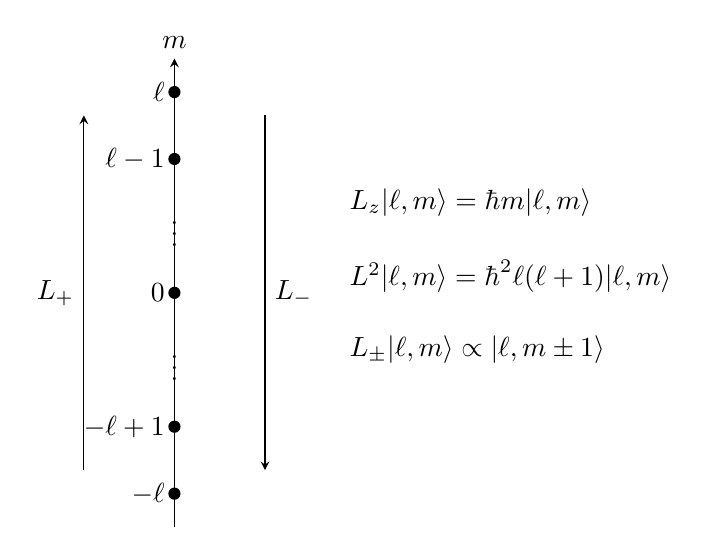
\begin{tikzpicture}[x=1cm,y=0.85cm,>=stealth]
\draw[->] (0,-3.5) -- (0,3.5) node[above] {$m$};

\fill (0,3) circle (2.2pt);
\fill (0,2) circle (2.2pt);
\fill (0,0) circle (2.2pt);
\fill (0,-2) circle (2.2pt);
\fill (0,-3) circle (2.2pt);

\node[left] at (0,3) {$\ell$};
\node[left] at (0,2) {$\ell-1$};
\node[left] at (0,0) {$0$};
\node[left] at (0,-2) {$-\ell+1$};
\node[left] at (0,-3) {$-\ell$};

\node at (0,1) {$\vdots$};
\node at (0,-1) {$\vdots$};

\draw[->] (-1.15,-2.65) -- (-1.15,2.65)
node[midway,left] {$L_+$};
\draw[->] (1.15,2.65) -- (1.15,-2.65)
node[midway,right] {$L_-$};

\node[anchor=west] at (2.1,1.35)
{$L_z|\ell,m\rangle=\hbar m|\ell,m\rangle$};
\node[anchor=west] at (2.1,0.25)
{$L^2|\ell,m\rangle=\hbar^2\ell(\ell+1)|\ell,m\rangle$};
\node[anchor=west] at (2.1,-0.85)
{$L_\pm|\ell,m\rangle\propto|\ell,m\pm1\rangle$};
\end{tikzpicture}\caption{Ein ganzzahliges orbitales Drehimpulsmultiplett. \(L_+\) und \(L_-\) ändern \(m\) jeweils um eins, während \(L^2\) im gesamten Multiplett den Wert \(\hbar^2\ell(\ell+1)\) behält.}\lectureframe{00:35:53}\end{figure}

\section{Das Zentralfeldproblem}

Betrachten wir
\begin{equation}
H=\frac{\mathbf p^2}{2m}+V(r),
\end{equation}
wobei \(V\) nur vom Abstand zum Ursprung abhängt. Aufgrund der Rotationssymmetrie ist der Drehimpuls erhalten. Klassisch haben \(\mathbf L\) einen festen Betrag und eine feste Richtung, sodass die Bahn in einer Ebene senkrecht zu \(\mathbf L\) verläuft. Die Bahn muss weder kreisförmig noch geschlossen sein.

Wir wählen die Koordinaten so, dass diese klassische Bahnebene die \(xy\)-Ebene ist, und zerlegen den Impuls in eine radiale und eine tangentiale Komponente:
\begin{equation}
\mathbf p^2=p_r^2+p_\theta^2.
\end{equation}
Da der Betrag des Drehimpulses
\begin{equation}
L=r p_\theta,
\end{equation}
beträgt, lässt sich der tangentiale Anteil schreiben als
\begin{equation}
p_\theta^2=\frac{L^2}{r^2}.
\end{equation}
Der Hamiltonoperator nimmt dann die Form an
\begin{equation}
H=\frac{p_r^2}{2m}+\frac{L^2}{2mr^2}+V(r).
\end{equation}
Bei festem \(L\) ist dies ein eindimensionales Problem in der Radialkoordinate mit dem effektiven Potential
\begin{equation}
V_{\mathrm{eff}}(r)=\frac{L^2}{2mr^2}+V(r).
\end{equation}
Der radiale Hamiltonoperator ist unten an der Tafel zu sehen.\footnote{Ausgangsbild: \texttt{\detokenize{lecture_03_frame_02.png}}, Vorlesungsvideo bei \(00{:}47{:}15\).}

\begin{figure}[htbp]\centering
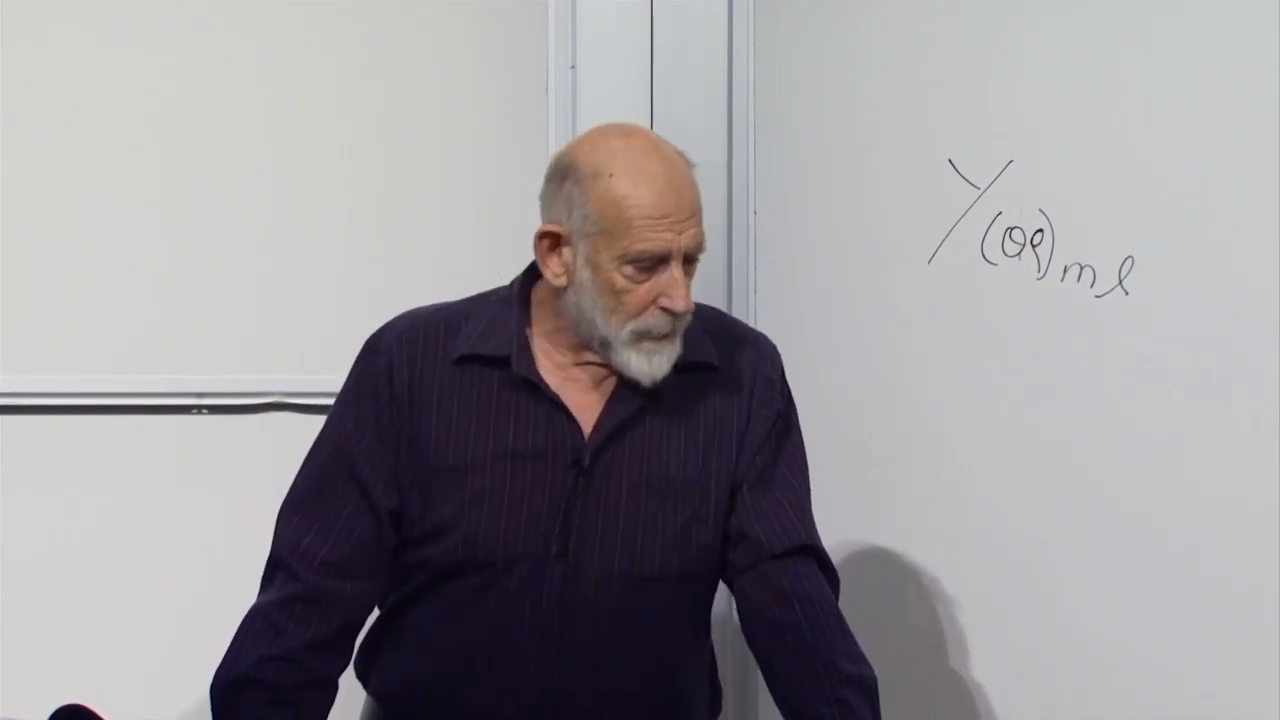
\includegraphics[width=0.9\linewidth]{lecture_03_frame_02.png}\caption{Bei festem klassischem Drehimpuls enthält der radiale Hamiltonoperator die radiale kinetische Energie, den Zentrifugalterm \(L^2/(2mr^2)\) und das Zentralpotential \(V(r)\).}\lectureframe{00:47:15}\end{figure}

Der Term \(1/r^2\) bildet die Zentrifugalbarriere. Sie steigt an, wenn sich das Teilchen dem Ursprung nähert, sodass die zugehörige Kraft nach außen gerichtet ist. Bei den hier betrachteten coulombartigen Anziehungspotentialen schwingt eine Bahn mit \(L\neq0\) um das Zentrum, statt es zu erreichen. Für \(L=0\) fehlt die Barriere.

Für das attraktive Coulombpotential gilt
\begin{equation}
V(r)=-\frac{\kappa}{r},
\end{equation}
Bei kleinen \(r\) dominiert der Zentrifugalterm, während der Coulombterm langsamer abfällt und bei großen \(r\) überwiegt. Für \(L\neq0\) besitzt die Summe ein Minimum. Die Bewegung am Minimum hat einen konstanten Radius und ist daher kreisförmig. Gebundene Bewegungen oberhalb des Minimums und unterhalb der Fluchtschwelle oszillieren zwischen einem minimalen und einem maximalen Radius; im Coulombproblem sind dies die radialen Oszillationen einer elliptischen Bahn.

\section{Die reduzierte Radialgleichung}

In der Quantenmechanik ist der Winkelanteil eines Zustands mit bestimmtem orbitalem Drehimpuls eine Kugelflächenfunktion. Wir schreiben den separierten Zustand als
\begin{equation}
\Psi_{n_r\ell m}(r,\theta,\phi)
=\frac{u_{n_r\ell}(r)}{r}\,
Y_{\ell m}(\theta,\phi).
\end{equation}
Der Winkeloperator \(L^2\) hat den Eigenwert
\begin{equation}
L^2Y_{\ell m}
=\hbar^2\ell(\ell+1)Y_{\ell m}.
\end{equation}
Für ein festes Wertepaar \(n_r,\ell\) kürzen wir \(u_{n_r\ell}(r)\) mit \(u(r)\) ab. Für die reduzierte Radialfunktion bleibt die Gleichung
\begin{equation}
\begin{aligned}
&-\frac{\hbar^2}{2m}\frac{d^2u}{dr^2}
+\frac{\hbar^2\ell(\ell+1)}{2mr^2}u(r)\\
&\qquad+V(r)u(r)=E_{n_r\ell}\,u(r).
\end{aligned}
\end{equation}

\editorialnote{Die rein eindimensionale Gleichung mit der zweiten Ableitung verwendet die reduzierte Radialfunktion \(u=rR\). Daher entspricht das \(\psi(r)\) in der dargestellten Vorlesungsgleichung \(u(r)\), während der gewöhnliche Radialfaktor in \(\Psi=R(r)Y_{\ell m}\) gleich \(R=u/r\) ist. Diese Konvention vermeidet, \(-i\hbar\,d/dr\) als eigenständigen hermiteschen Radialimpulsoperator im dreidimensionalen radialen Hilbertraum zu behandeln.}

Die reduzierte Radialgleichung ist unten an der Tafel zu sehen.\footnote{Ausgangsbild: \texttt{\detokenize{lecture_03_frame_03.png}}, Vorlesungsvideo bei \(00{:}54{:}32\).}

\begin{figure}[htbp]\centering
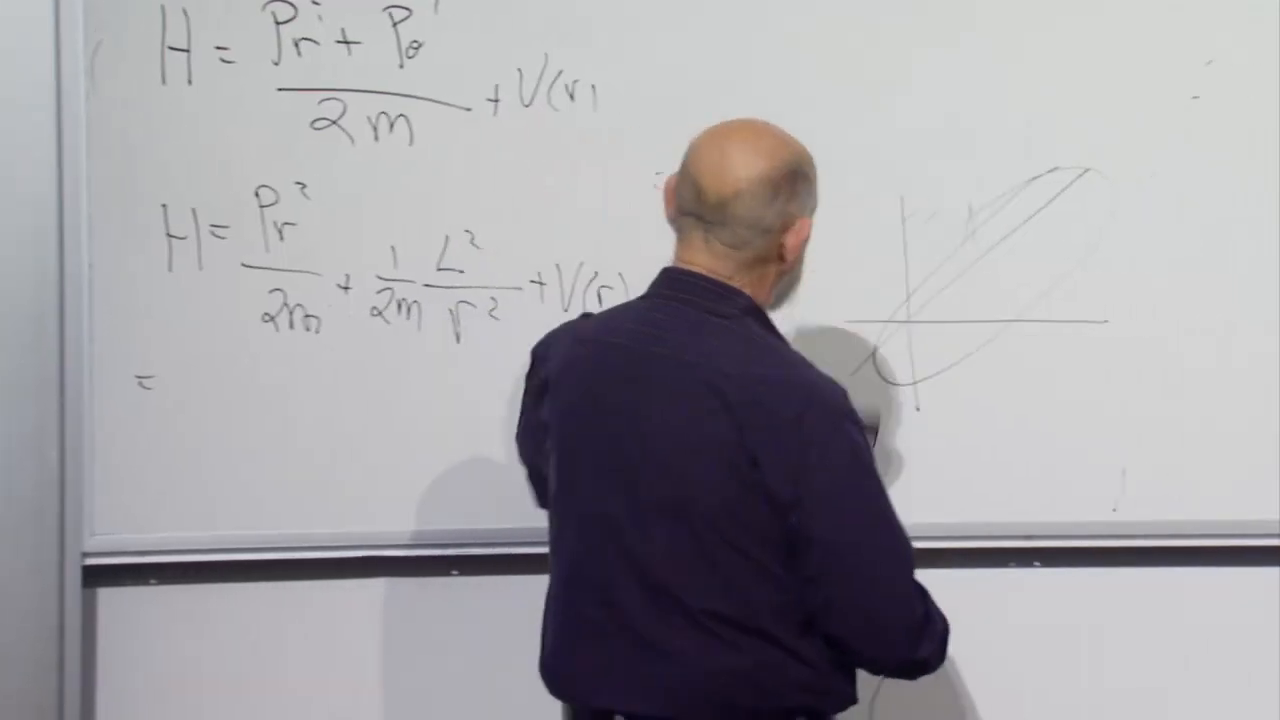
\includegraphics[width=0.9\linewidth]{lecture_03_frame_03.png}\caption{Bei festem \(\ell\) erfüllt die reduzierte Radialwellenfunktion eine eindimensionale Schr\"odinger-Gleichung mit einem Zentrifugalterm proportional zu \(\ell(\ell+1)/r^2\).}\lectureframe{00:54:32}\end{figure}

Die dreidimensionale Winkelstruktur ist im Parameter \(\ell\) zusammengefasst. Die magnetische Quantenzahl \(m\) tritt in der Radialgleichung nicht auf.

\begin{classroomqa}\lecturetimestamp{00:55:34}\audiencequestion{Haben die \(2\ell+1\) magnetischen Zustände bei gegebenem \(\ell\) dieselbe Energie?}\lecturerresponse{Ja, sofern auch der radiale Eigenzustand festgehalten wird. Bei jedem gewählten \(u_{n_r\ell}\) haben alle Werte \(m=-\ell,\ldots,\ell\) dieselbe Energie, weil \(m\) nicht in die Radialgleichung eingeht. Verschiedene radiale Eigenzustände bei demselben \(\ell\) haben im Allgemeinen unterschiedliche Energien.}\end{classroomqa}

\begin{classroomqa}\lecturetimestamp{00:56:03}\audiencequestion{Warum darf \(L^2\) durch \(\hbar^2\ell(\ell+1)\) ersetzt werden, und wie hängt \(\ell\) mit den erlaubten Werten von \(m\) zusammen?}\lecturerresponse{Die Zahl \(\ell\) kennzeichnet ein Drehimpulsmultiplett und ist der größte darin auftretende \(m\)-Wert. Alle Zustände dieses Multiplets haben denselben \(L^2\)-Eigenwert, nämlich \(\hbar^2\ell(\ell+1)\); dieser Eigenwert wird daher in die Radialgleichung eingesetzt.}\end{classroomqa}

Die expliziten Lösungen mit speziellen Funktionen werden für die vorliegende Argumentation nicht benötigt. Entscheidend ist, wie die Lösungen angeordnet sind.

\section{Radiale Knoten und Energieniveaus}

Bei festem \(\ell\) ist die reduzierte Radialgleichung ein gewöhnliches eindimensionales Eigenwertproblem. Seine gebundenen Zustände sind nach der Zahl ihrer inneren Knoten geordnet. Der niedrigste radiale Zustand hat keinen inneren Knoten, der nächste einen und der darauffolgende zwei. Eine größere Knotenzahl bedeutet, dass sich die Wellenfunktion schneller ändert; dadurch ist der Impuls größer und folglich auch die kinetische Energie.

Jeder Wert von \(\ell\) definiert einen anderen radialen Operator, denn der Zentrifugalterm ändert sich mit \(\ell\). Somit bilden \(\ell=0,1,2,\ldots\) getrennte radiale Niveautürme. Der positive Zentrifugalterm verschiebt die Niveaus nach oben, wenn der Drehimpuls zunimmt. Jeder radiale Eigenwert bei festem \(\ell\) gehört zu einem magnetischen Multiplett der Dimension
\begin{equation}
2\ell+1.
\end{equation}
Die Niveaus mit \(\ell=0\) sind Singuletts, diejenigen mit \(\ell=1\) Tripletts und diejenigen mit \(\ell=2\) Quintetts. Dies sind die durch die Rotationssymmetrie gewährleisteten Entartungen; eine zusätzliche Symmetrie kann auch Zustände mit verschiedenen Werten von \(\ell\) entarten lassen.

Für Potentiale vom Typ eines Atompotentials, die die Bedingung \(V(r)\to0\) bei großen \(r\) erfüllen, liegt die Fluchtschwelle üblicherweise bei \(E=0\). Die Zustände mit negativer Energie bilden das diskrete gebundene Spektrum. Bei und oberhalb von \(E=0\) liegt das Streukontinuum vor. Diese Aussage hängt vom Verhalten des Potentials bei großen \(r\) ab und gilt nicht für ein einschließendes Zentralpotential.

\section{Die besondere Coulomb-Entartung}

Beim exakten nichtrelativistischen Coulombpotential fallen zusätzlich bestimmte Energieniveaus zusammen. Der niedrigste radiale Zustand mit \(\ell=1\) hat dieselbe Energie wie der erste angeregte Zustand mit \(\ell=0\). Der nächsthöhere Zustand mit \(\ell=1\) fällt mit dem zweiten angeregten Zustand mit \(\ell=0\) zusammen; auch der niedrigste Zustand mit \(\ell=2\) gehört zu dieser Gruppe. Das Muster setzt sich bei den höheren radialen und Drehimpulstürmen fort.

\begin{classroomqa}\lecturetimestamp{01:09:57}\audiencequestion{Deutet diese zusätzliche Coulomb-Entartung auf eine weitere Symmetrie hin?}\lecturerresponse{Ja. Sie beruht auf einer ungewöhnlichen zusätzlichen Symmetrie des exakten Coulombpotentials. Kleine Änderungen des Potentials heben das Zusammenfallen der Niveaus auf; die Herleitung wird hier nicht behandelt.}\end{classroomqa}

Die daraus resultierenden Entartungsgrade der orbitalen Schalen sind
\begin{equation}
1,\qquad 4,\qquad 9,\qquad 16,\qquad \ldots
\end{equation}
noch ohne Berücksichtigung des Elektronenspins.

\begin{classroomqa}\lecturetimestamp{01:11:46}\audiencequestion{Gilt diese Entartung für Wasserstoff oder nur für das ideale Coulombproblem?}\lecturerresponse{Für Wasserstoff gilt sie mit sehr guter Näherung, aber nicht exakt. Relativistische Korrekturen und die endliche Größe des Atomkerns stören das ideale Coulombmuster.}\end{classroomqa}

Ein punktförmiger Kern erzeugt ein exaktes \(1/r\)-Potential. Ist die Kernladung über ein kleines Volumen verteilt, entsteht ein leicht anderes Potential, wenn das Elektron in dieses Volumen eindringt. Selbst diese kleine Abweichung hebt einen Teil der besonderen Entartung auf.

Auch der Spin wurde bisher nicht berücksichtigt. Bezieht man die beiden Elektronenspinzustände ein, verdoppeln sich die Schalenbesetzungszahlen zu
\begin{equation}
2,\qquad 8,\qquad 18,\qquad 32,\qquad \ldots
\end{equation}
bevor die weiteren Aufspaltungen einer vollständigeren atomaren Beschreibung berücksichtigt werden.

\section{Noch einmal zur kartesischen Gleichung}

Die Gleichung, von der das Radialproblem ausging, ist die dreidimensionale zeitunabhängige Schr\"odinger-Gleichung
\begin{equation}
\begin{aligned}
-\frac{\hbar^2}{2m}\nabla^2\Psi+V(r)\Psi&=E\Psi,\\
\nabla^2&=\frac{\partial^2}{\partial x^2}
+\frac{\partial^2}{\partial y^2}
+\frac{\partial^2}{\partial z^2},\\
r&=\sqrt{x^2+y^2+z^2}.
\end{aligned}
\end{equation}
Wir wechseln zu Radial- und Winkelkoordinaten und wählen einen Eigenzustand von \(L^2\).
Ersetzt man \(L^2\) durch \(\hbar^2\ell(\ell+1)\), so wird die partielle Differentialgleichung auf die oben angegebene gewöhnliche Radialgleichung reduziert.

\begin{classroomqa}\lecturetimestamp{01:16:42}\audiencequestion{Lässt sich aus Abweichungen vom idealen Coulombspektrum die Größe des Atomkerns bestimmen?}\lecturerresponse{Nicht durch diesen einfachen Vergleich. Andere Korrekturen sind viel größer und müssen zuerst berücksichtigt werden. Die Kerngröße wird hier erwähnt, weil sie unmittelbar ein Beispiel für eine Abweichung vom Punkt-Coulombpotential liefert.}\end{classroomqa}

\begin{classroomqa}\lecturetimestamp{01:17:09}\audiencequestion{Was ist der wichtigste Unterschied zwischen den klassischen und quantenmechanischen Drehimpulstermen?}\lecturerresponse{Klassisch ist \(L^2\) einfach das Quadrat des Betrags eines erhaltenen Vektors. In einem quantenmechanischen orbitalen Multiplett ist der Eigenwert \(\hbar^2\ell(\ell+1)\) und nicht einfach \(\hbar^2\ell^2\). Der zusätzliche Term ergibt sich aus der Nichtvertauschbarkeit der Drehimpulskomponenten.}\end{classroomqa}

\begin{classroomqa}\lecturetimestamp{01:17:58}\audiencequestion{Haben die Wellenfunktionen gebundener Zustände kompakten Träger?}\lecturerresponse{Nein. Sie erstrecken sich beliebig weit vom Zentrum weg. Bei den hier betrachteten gebundenen Atomzuständen fallen sie bei großen Abständen exponentiell ab. Die Wahrscheinlichkeit wird dadurch vernachlässigbar klein, verschwindet aber nicht außerhalb irgendeines endlichen Radius.}\end{classroomqa}

\begin{classroomqa}\lecturetimestamp{01:18:48}\audiencequestion{Was geschieht mit dem stabilen Punkt, wenn \(\ell=0\) die Zentrifugalmulde beseitigt?}\lecturerresponse{Ein Minimum, das aus dem Zusammenspiel von Zentrifugalbarriere und Anziehung entsteht, gibt es dann nicht mehr. Im idealisierten Punkt-Coulombpotential bewegt sich das klassische Teilchen auf das singuläre Zentrum zu. Quantenmechanisch kann der niedrigste Zustand nicht zugleich eine exakt bestimmte Position im Zentrum und einen Impuls von null haben; daher weist die Wellenfunktion des niedrigsten Zustands eine endliche räumliche Ausdehnung auf.}\end{classroomqa}

\editorialnote{Bei einem regulären Zentralpotential kann eine klassische Bahn mit Drehimpuls null durch den Ursprung weiterlaufen. Beim idealen Punkt-Coulombpotential ist \(r=0\) dagegen eine Kollisionssingularität; die Fortsetzung der klassischen Bahn erfordert eine zusätzliche Vorschrift.}

Bei der klassischen Reduktion wurde eine einzelne Bahn in eine Ebene gelegt. Dieser Schritt lässt sich jedoch nicht auf dieselbe Weise auf eine quantenmechanische Wellenfunktion anwenden. Ein orbitaler Quantenzustand erstreckt sich über den dreidimensionalen Raum. Der vollständige Winkeloperator lautet \(L^2=L_x^2+L_y^2+L_z^2\), und sein Eigenwert bewahrt das dreidimensionale Ergebnis \(\hbar^2\ell(\ell+1)\).

\begin{classroomqa}\lecturetimestamp{01:21:30}\audiencequestion{Wie kann das quantenmechanische Problem dreidimensional bleiben, nachdem die klassische Bahn in eine Ebene gelegt wurde?}\lecturerresponse{Nur die klassische Bahn wurde durch eine Koordinatenwahl in eine feste Ebene gelegt, deren Normale parallel zum erhaltenen Drehimpulsvektor ist. Eine quantenmechanische Wellenfunktion nimmt den dreidimensionalen Raum ein. Die übrigen Drehimpulskomponenten bleiben über \(L^2\) erhalten. Deshalb enthält die Radialgleichung \(\ell(\ell+1)\) und nicht nur das Quadrat einer einzelnen Komponente.}\end{classroomqa}

\begin{classroomqa}\lecturetimestamp{01:22:54}\audiencequestion{Gibt es in jedem quantenmechanischen Problem Erzeugungs- und Vernichtungsoperatoren?}\lecturerresponse{Nein. Sie treten in besonders günstigen Fällen auf. Der Drehimpuls ist ein solcher Fall, der harmonische Oszillator ein weiterer. Der Oszillator ist besonders nützlich, weil die Bewegung in der Nähe eines stabilen Gleichgewichts so häufig näherungsweise harmonisch ist. Dazu gehören kleine radiale Schwingungen nahe dem Minimum eines effektiven Potentials.}\end{classroomqa}

An dieser Stelle wird das Atomproblem zurückgestellt. Als nächstes Beispiel folgt der harmonische Oszillator, dessen Spektrum sich mithilfe von Leiteroperatoren bestimmen lässt.

\section{Kleine Schwingungen und der harmonische Oszillator}

In der Nähe eines stabilen Gleichgewichts führt eine hinreichend kleine Auslenkung häufig zu harmonischer Bewegung. Das effektive Radialpotential bei von null verschiedenem Drehimpuls liefert ein Beispiel dafür: Nahe dem Tiefpunkt seiner Mulde ist die radiale Bewegung näherungsweise harmonisch.

Betrachten wir einen eindimensionalen Oszillator mit Einheitsmasse. Die Auslenkung aus der Gleichgewichtslage sei \(x\), und die Federkonstante schreiben wir als \(k=\omega^2\). Der klassische Hamiltonian lautet
\begin{equation}
H=\frac{p^2}{2}+\frac{\omega^2x^2}{2}.
\end{equation}
Aus den Hamilton-Gleichungen folgt
\begin{equation}
\dot{x}=\frac{\partial H}{\partial p}=p,
\qquad
\dot{p}=-\frac{\partial H}{\partial x}=-\omega^2x,
\end{equation}
und damit
\begin{equation}
\ddot{x}=-\omega^2x.
\end{equation}
Somit ist \(\omega\) die klassische Schwingungsfrequenz.

\section{Faktorisierung und Nullpunktsenergie}

Quantenmechanisch gilt
\begin{equation}
[x,p]=i\hbar.
\end{equation}
Der Hamiltonoperator ist eine Summe von Quadraten, was eine Faktorisierung nahelegt:
\begin{align}
\frac{1}{2}(p+i\omega x)(p-i\omega x)
&=\frac{1}{2}\left(p^2+\omega^2x^2+i\omega[x,p]\right) \\
&=\frac{1}{2}\left(p^2+\omega^2x^2-\hbar\omega\right).
\end{align}
Daraus folgt
\begin{equation}
H=\frac{1}{2}(p+i\omega x)(p-i\omega x)
+\frac{1}{2}\hbar\omega.
\end{equation}
Der additive Term \(\hbar\omega/2\) ist die Nullpunktsenergie.

Klassisch würde die niedrigste Energie bei \(x=p=0\) auftreten. Quantenmechanisch kann kein Zustand sowohl einen exakt festgelegten Ort als auch einen exakt festgelegten Impuls gleich null haben. Zudem sind die beiden Terme \(p^2/2\) und \(\omega^2x^2/2\) positiv und können einander nicht aufheben. Eine von null verschiedene Grundzustandsenergie ist daher unvermeidlich.

Für die Berechnung mit den Leiteroperatoren kann die gemeinsame additive Konstante vorübergehend beiseitegelassen und am Ende wieder hinzugefügt werden.

\begin{classroomqa}\lecturetimestamp{01:36:10}\audiencequestion{Lässt sich aus dem positiven Vorzeichen des Nullpunktsenergie-Terms noch etwas Weiteres schließen?}\lecturerresponse{Der Hamiltonoperator des Oszillators ist positiv: Er ist eine Summe positiver Quadrate, daher kann seine Energie nicht negativ sein.}\end{classroomqa}

\section{Die Leiter des Oszillators}

Wir führen die dimensionslosen Operatoren ein.\footnote{In \(01{:}37\)--\(01{:}42\) wird mit \(\hbar=1\) gerechnet. In diesen normierten Definitionen wird der Faktor \(\hbar\) wieder eingesetzt, sodass \(A_\pm\) dimensionslos sind und ihr Kommutator eins beträgt.}
\begin{equation}
A_+=\frac{p+i\omega x}{\sqrt{2\hbar\omega}},
\qquad
A_-=\frac{p-i\omega x}{\sqrt{2\hbar\omega}}.
\end{equation}
Sie sind zueinander adjungiert:
\begin{equation}
A_+^\dagger=A_-.
\end{equation}
Ihr Kommutator lautet
\begin{align}
[A_-,A_+]
&=\frac{1}{2\hbar\omega}
\left([p,i\omega x]+[-i\omega x,p]\right) \\
&=1.
\end{align}

Wir definieren
\begin{equation}
N=A_+A_-.
\end{equation}
Dann lautet der Hamiltonoperator
\begin{equation}
H=\hbar\omega\left(N+\frac{1}{2}\right).
\end{equation}
Damit reduziert sich die Bestimmung des Energiespektrums auf die Bestimmung der Eigenwerte von \(N\).

Es sei
\begin{equation}
N|n\rangle=n|n\rangle.
\end{equation}
Die Kommutatoren mit \(N\) lauten wie folgt.\footnote{Die Zwischenschritte bei \(01{:}45{:}37\)--\(01{:}48{:}10\) lassen sich unmittelbar aus den angegebenen Relationen \(N=A_+A_-\) und \([A_-,A_+]=1\) rekonstruieren.}
\begin{align}
[N,A_+]
&=A_+[A_-,A_+]=A_+, \\
[N,A_-]
&=[A_+,A_-]A_-=-A_-.
\end{align}
Daraus folgt
\begin{align}
N\bigl(A_+|n\rangle\bigr)
&=(n+1)A_+|n\rangle, \\
N\bigl(A_-|n\rangle\bigr)
&=(n-1)A_-|n\rangle.
\end{align}
Somit erhöht \(A_+\) einen Eigenwert von \(N\) um eins und \(A_-\) verringert ihn um eins, sofern der resultierende Vektor nicht verschwindet.

Der Operator \(N\) ist nichtnegativ:
\begin{equation}
\langle\psi|N|\psi\rangle
=\langle\psi|A_+A_-|\psi\rangle
=\|A_-|\psi\rangle\|^2
\geq0.
\end{equation}
Der Absenkprozess kann daher nicht zu negativen Eigenwerten führen. Bei einem untersten Zustand \(|b\rangle\) muss er enden:
\begin{equation}
A_-|b\rangle=0.
\end{equation}

Bei normierten Eigenzuständen sind die Koeffizienten der Leiter durch ihre Normen festgelegt:
\begin{align}
\|A_-|n\rangle\|^2
&=\langle n|A_+A_-|n\rangle=n, \\
\|A_+|n\rangle\|^2
&=\langle n|A_-A_+|n\rangle=n+1.
\end{align}
Die Phasen lassen sich daher so wählen, dass
\begin{equation}
A_-|n\rangle=\sqrt{n}\,|n-1\rangle,
\qquad
A_+|n\rangle=\sqrt{n+1}\,|n+1\rangle.
\end{equation}

\begin{classroomqa}\lecturetimestamp{01:52:42}\audiencequestion{Wenn \(A_-\) einen Zustand absenkt und \(A_+\) ihn wieder anhebt, wie ergibt \(A_+A_-\) dann den Eigenwert \(n\)?}\lecturerresponse{Die Wirkung der Leiter enthält Normierungsfaktoren. Die Anwendung von \(A_-\) liefert den Faktor \(\sqrt n\), und bei der anschließenden Anwendung von \(A_+\) auf den resultierenden Zustand kommt ein weiterer Faktor \(\sqrt n\) hinzu. Ihr Produkt ist \(n\).}\end{classroomqa}

Tatsächlich gilt
\begin{equation}
A_+A_-|n\rangle
=\sqrt n\,A_+|n-1\rangle
=n|n\rangle.
\end{equation}

\begin{classroomqa}\lecturetimestamp{01:55:52}\audiencequestion{Muss der niedrigste Eigenwert von \(N\) null sein, oder könnte er positiv sein?}\lecturerresponse{Er muss null sein, und das Spektrum von \(N\) besteht aus den nichtnegativen ganzen Zahlen. Der Beweis für diesen Endpunkt wurde noch nicht erbracht.}\end{classroomqa}

\editorialnote{Sei \(|b\rangle\) ein Zustand mit dem niedrigsten Eigenwert. Da der Absenkprozess enden muss, gilt \(A_-|b\rangle=0\). Daraus folgt unmittelbar \(N|b\rangle=A_+A_-|b\rangle=0\); der niedrigste Eigenwert von \(N\) ist also null.}

Ausgehend von diesem untersten Zustand erhalten wir durch wiederholte Anwendung von \(A_+\)
\begin{equation}
n=0,1,2,\ldots.
\end{equation}
Nach Wiederherstellung des additiven Nullpunktsenergie-Terms lauten die Oszillatorenergien
\begin{equation}
E_n=\hbar\omega\left(n+\frac{1}{2}\right),
\qquad n=0,1,2,\ldots.
\end{equation}

Die Oszillatoralgebra wird weiterentwickelt und zur Lösung anderer quantenmechanischer Probleme eingesetzt.